\section{Sensorik und Sicherheitstechnik \textcolor{gray}{(Elena Widmann)}}

\subsection{Aufgabenstellung}

\subsection{Sensorik}

\subsubsection{Endschalter}
Beim Verplanen der Endschalter ist zwischen Software- und Hardware-Endschalter zu unterscheiden. Die Software-Endschalter begrenzen den Arbeitsbereich der Achse und sollten innerhalb des Bereichs der Hardware-Endschalter parametriert werden. Ihre Positionen werden direkt im Siemens TIA-Portal eingestellt und können falls notwendig einfach auf die aktuelle Geschwindigkeit angepasst werden. Werden die Software-Endschalter angefahren wird der Technologiealarm 533 ausgelöst und die Dynamikwerte werden gestoppt, das Technologieobjekt bleibt hierbei freigegeben. Werden sie jedoch überfahren wird das Technologieobjekt gesperrt. \\
Die Hardware-Endschalter begrenzen den maximal zulässigen Verfahrensbereich der Achse. Bei ihnen wird nicht unterschieden, ob die Endschalter angefahren oder überfahren werden. Beim Anfahren der Schalter wird der Technologiealarm 531 ausgelöst. Er sperrt das Technologieobjekt und muss, bevor der Auslösebereich der Hardware-Endschalter wieder verlassen werden kann, quittiert werden. \cite{axis_manual}\\
Auf jeder der drei Achsen vom AFSS und auf dem Querförderer müssen Hardware-Endschalter montiert werden. Die Auswahl begrenzte sich hierbei auf die uns zur Verfügung gestellten Sensoren, welche ihren Funktion entsprechend auf den verschiedenen Positionen eingebaut werden.

\paragraph{Positionsschalter mit Rollhebel}
An der x-Achse werden als Hardware-Endschalter Positionsschalter mit Rollhebel verwendet. Davon besitzen drei jeweils einem Öffner- und einen Schließerkontakt \cite{schmersal_3}, wohingegen einer der Endschalter aus zwei Öffnerkontakten besteht. \cite{schmersal_1} Um Einheitlich zu bleiben und da es sicherheitstechnisch auch von Vorteil ist (Drahtbruchsicherheit) verwenden wir jeweils einen der Öffnerkontakte der Endschalter.

\paragraph{Induktive Endschalter}
\begin{wrapfigure}{r}{0.3\textwidth}
    \vspace{-20px}
    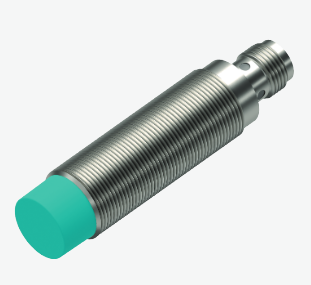
\includegraphics[width=0.3\textwidth]{Sensors/Induktiver_Sensor.png}
    \caption{Induktiver Sensor \cite{induktiv_sensor}}
\end{wrapfigure}
Als Hardware-Endschalter an der y-Achse werden induktive Sensoren verwendet. Sie funktionieren so, dass durch eine Spule ein Magenetfeld erzeugt wird, welches dann in einem sich dem Sensor frontseitig nähernden elektrisch leitendem Material Wirbelströme erzeugt. Dadurch verändert sich das Magnetfeld und die Kontakte des induktive Sensors werden über einen Schmitt-Trigger geschaltet. Die Sensoren besitzen jeweils einen Öffner- und einen Schließerkontakt, wir verwenden jedoch ersteres um Drahtbruchsicherheit zu gewährleisten.

\paragraph{Endtaster}
An der z-Achse und am Querförderer werden mechanische Endtaster verwendet. Auf einem Endtaster befindet sich ein Schließerkontakt in Form eines Tasters, welcher durch anfahren geschaltet wird.

\subsubsection{Referenztaster}

\subsubsection{Lichttaster}

\subsubsection{Barcode-Scanner}

\subsection{AS-Interface}

\subsubsection{Allgemeines}

\subsubsection{Programmierung im TIA-Portal}

\subsubsection{Unterverteilerplatine}


\subsection{Sicherheitstechnik}
\subsubsection{Grundanforderungen und Planung}
\subsubsection{Realisierung}